\subsubsection{Calculation} \label{sec:methodology}
%How, then, can \xQ{} be calculated? 
Following the above discussion, a surrogate model \surrogate{} can be learned,  as shown in Fig.~\ref{fig:sq_v3} (right), to predict the reward distribution \rwdstarapprox{} of the `trusted' reference solver \solvestar{} on task \task{} (which ideally comes close to approximating the optimal $\pi$ or converges to it with unlimited computing resources). The candidate solver \solve{} must then be evaluated online with respect to the trusted solver \solvestar{}. This is done by comparing \rwdstarapprox{} (the predicted performance of \solvestar{} on task \task) and \rwd{} (the simulated performance of solver \solve{} on task \task). %% as illustrated in Fig.~\ref{fig:sq_v3} (right).
This approach is inspired by empirical hardness modeling techniques \cite{Leyton-Brown2009-yr}, which use surrogate models to predict the actual run time of NP-complete problem solvers. 
Figure~\ref{fig:sq_v3} (left) illustrates some of the key quantities involved in calculating \xQ{}. The basic premise is to evaluate a scaled version of the Hellinger distance between the difference between the reward distributions of the trusted ($T$) and candidate ($C$) solvers, while taking into account the overall range of rewards of the trusted solver over many tasks. %This is discussed further in \cite{Israelsen2018-qz}.
For brevity, here we will only present the key equations developed in detail in \cite{Israelsen2018-qz} for calculating \xQ{}, 
\begin{align}
    x_{Q} = \frac{2}{1+\exp(-\text{q}/5)}, \ \ \
    f = \frac{\Delta \mu}{r_H - r_L}, \ \ \
    %\label{eq:SQ}, \ \ \
    \text{q} = \text{sgn}(\Delta \mu)f^{\alpha}\sqrt{H^{2}(T,C)} \label{eq:SQ} %\label{eq:q}
\end{align}
%\nisar{WHAT IS H?? other vars??}
where $H^2(T,C)$ is the Hellinger distance between the $p(R_{\infty})$ pdfs $T$ for \solvestar{} and $C$ for \solve{}; $\Delta \mu$ is the difference in the means of these pdfs; $\mbox{sgn}$ is the signum function; $r_H$ and $r_L$ are largest and smallest $R_{\infty}$ values observed in the \solvestar{} training set; and the $\alpha$ is a tuning parameter to adjust the steepness
of \xQ{} vs. q over the range 0 (total lack of confidence in \solve{} relative to \solvestar{}) to 2 (complete confidence in \solve{} relative to \solvestar{}), with the midpoint at 1 (equal confidence in \solve{} relative to \solvestar{}). 
% \begin{figure}[tbp]
%     \centering
%     \begin{subfigure}[c]{0.50\linewidth}
%         \centering
%         
\includegraphics[width=0.55\linewidth]{Figures/SQ_train.png}
%         \vfill
%         \caption{Offline Training}
%         \label{fig:sq_train}
%     \end{subfigure}%
%     \hfill
%     \begin{subfigure}[c]{0.50\linewidth}
%         \centering
%         
\includegraphics[width=0.75\linewidth]{Figures/SQ_test.png}
%         \caption{Online Deployment}
%         \label{fig:sq_test}
%     \end{subfigure} 
%     \caption{Depiction of the training phase of the surrogate function \surrogate, and the test, or online deployment, phase where \xQ{} is calculated.}
%     \label{fig:sq_test_train}
% \end{figure}
%
%
%\subsubsection{Numerical Examples}
%\brett{this may not be \emph{necessary}, but we mentioned in the submitted abstract that we have `numerical experiments' that show \xQ{} is useful. It would be helpful to make this as short as possible}. 
%\nisar{explanation of values need to edited for consistency...range here is 0 to 2...}
%A toy example is useful in evaluating whether \xQ{} yields expected/desirable results. 
Figure~\ref{fig:sq_thry1} illustrates the expected reward (with uncertainty) for a trusted solver \solvestar{} given a specific, generic, task/solver parameter, as well as that of a `candidate' solver \solve. Different points of interest (indicating specific values of the task parameter) are highlighted by a star. The table on the side shows the values of \xQ{} calculated for different cases. At point B the candidate solver has a lower expected reward than the trusted solver and a higher variance than the trusted solver. Intuitively \xQ{} should be less than one. As shown when $r=5$ (i.e. $r_H-r_L=5$, the global reward range is `large') $x_Q=0.667$ which indicates that the candidate solver is marginally less capable than the trusted solver, and when $r=0.05$ then $x_Q=0.002$ indicates that \solve{} is much less capable than \solvestar. At point C, \solve{} has higher expected reward than \solvestar, but a larger variance. Intuitively expect \xQ{} of \solve{} to be a little greater than one; in fact when $r=5$, $x_Q=1.095$. As the global reward range $r$ decreases the difference in capability between \solve{} and \solvestar{} increases with $x_Q=1.995$ at $r=0.005$. These calculations indicate that \xQ{} performs as expected. In Sec.~\ref{sec:exp_results} a more realistic scenario is considered, and the impact of self-confidence reporting on human user task delegation is tested experimentally. 

\begin{figure}[tbp]
    \centering
    \begin{subfigure}[c]{0.65\linewidth}
        \centering
        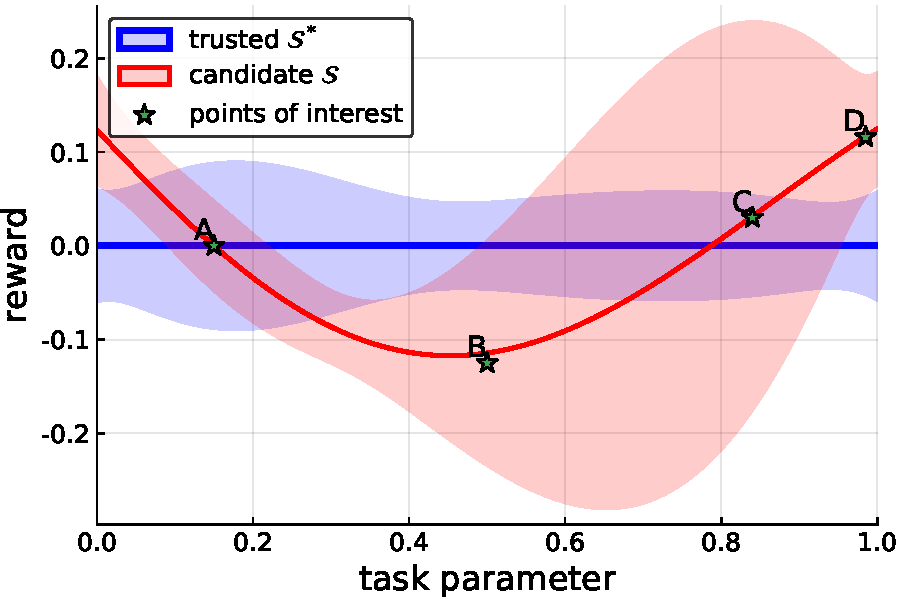
\includegraphics[width=0.7\linewidth]{Figures/p1.pdf}
        \vfill
        % \caption{tst}
        % \label{fig:}
    \end{subfigure}%
    \hfill
    \begin{subfigure}[t]{0.35\linewidth}
        \centering
        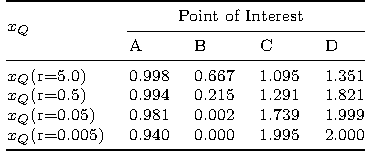
\includegraphics[width=1.0\linewidth]{Figures/p1_table.pdf}
        % \caption{Candidate solver depth 1}
        % \label{fig:med_roadnet}
    \end{subfigure} 
    \caption{\xQ{} assessments on synthetic $p(R_{\infty})$ distributions for \solvestar{} and \solve{}.} %Points of interest indicated by a star.}
    \label{fig:sq_thry1}
\end{figure}
